% TEMPLATE for Usenix papers, specifically to meet requirements of
%  USENIX '05
% originally a template for producing IEEE-format articles using LaTeX.
%   written by Matthew Ward, CS Department, Worcester Polytechnic Institute.
% adapted by David Beazley for his excellent SWIG paper in Proceedings,
%   Tcl 96
% turned into a smartass generic template by De Clarke, with thanks to
%   both the above pioneers
% use at your own risk.  Complaints to /dev/null.
% make it two column with no page numbering, default is 10 point

% Munged by Fred Douglis <douglis@research.att.com> 10/97 to separate
% the .sty file from the LaTeX source template, so that people can
% more easily include the .sty file into an existing document.  Also
% changed to more closely follow the style guidelines as represented
% by the Word sample file.

% Note that since 2010, USENIX does not require endnotes. If you want
% foot of page notes, don't include the endnotes package in the
% usepackage command, below.

% This version uses the latex2e styles, not the very ancient 2.09 stuff.
\documentclass[letterpaper,twocolumn,10pt]{article}
\usepackage{usenix,epsfig,endnotes}
\usepackage{cite}
\usepackage{amsmath,amssymb,amsfonts}
\usepackage{algorithmic}
\usepackage{graphicx}
\usepackage{textcomp}
\usepackage{amsfonts,amsthm,amsmath,amssymb}
\usepackage{hyperref}
\usepackage{framed}
\usepackage{array}
\usepackage{epsfig}
\usepackage{tikz}
\usepackage{enumitem}
\usepackage{url}
\usepackage{graphicx}
\usepackage{pgfplotstable}
\usepackage{pgfplots}
\usepackage[small,compact]{titlesec}
\usepackage{microtype}
\usepackage{titling}
\usepackage{tabularx}
\usetikzlibrary{positioning}
\def\BibTeX{{\rm B\kern-.05em{\sc i\kern-.025em b}\kern-.08em
    T\kern-.1667em\lower.7ex\hbox{E}\kern-.125emX}}

\newcommand{\ignore}[1]{}

\newtheorem{theorem}{Theorem}
\newtheorem{definition}[theorem]{Definition}
\newcommand{\getsR}{\overset{\$}{\leftarrow}}
\def\name/{ObliDB}

\pgfplotsset{width=6cm,compat=1.9}

% Alter some LaTeX defaults for better treatment of figures:
    % See p.105 of "TeX Unbound" for suggested values.
    % See pp. 199-200 of Lamport's "LaTeX" book for details.
    %   General parameters, for ALL pages:
    \renewcommand{\topfraction}{0.9}	% max fraction of floats at top
    \renewcommand{\bottomfraction}{0.8}	% max fraction of floats at bottom
    %   Parameters for TEXT pages (not float pages):
    \setcounter{topnumber}{2}
    \setcounter{bottomnumber}{2}
    \setcounter{totalnumber}{4}     % 2 may work better
    \setcounter{dbltopnumber}{2}    % for 2-column pages
    \renewcommand{\dbltopfraction}{0.9}	% fit big float above 2-col. text
    \renewcommand{\textfraction}{0.07}	% allow minimal text w. figs
    %   Parameters for FLOAT pages (not text pages):
    \renewcommand{\floatpagefraction}{0.9}	% require fuller float pages
	% N.B.: floatpagefraction MUST be less than topfraction !!
    \renewcommand{\dblfloatpagefraction}{0.9}	% require fuller float pages

	% remember to use [htp] or [htpb] for placement

	\setlength{\abovecaptionskip}{2pt}
	\setlength{\belowcaptionskip}{-9pt}

\begin{document}

%don't want date printed
\date{\vspace{-0.9cm}}

\setlength{\droptitle}{-1.1cm}

%make title bold and 14 pt font (Latex default is non-bold, 16 pt)
%\title{\Large \bf \name/: A Cloud Database with Access Pattern Leakage Protection}
%\title{\Large \bf \name/: An Oblivious SQL Database for Cloud Computing}
\title{\Large \bf An Oblivious General-Purpose SQL Database for Cloud Computing\vspace{-0.1cm}}

\author{\emph{Paper \# XXX}}

\ignore{
%for single author (just remove % characters)
\author{
{\rm Your N.\ Here}\\
Your Institution
\and
{\rm Second Name}\\
Second Institution
% copy the following lines to add more authors
% \and
% {\rm Name}\\
%Name Institution
} % end author
}
\maketitle

% Use the following at camera-ready time to suppress page numbers.
% Comment it out when you first submit the paper for review.
%\thispagestyle{empty}

% TODO: limitations (not distributed)

\subsection*{Abstract}
We present \name/, a secure SQL database for the public cloud that supports both transactional and analytics workloads and protects against access pattern leakage.
With many database workloads moving to the cloud, there is significant interest in securing them.
Hardware enclaves offer a strong practical foundation towards this goal by providing encryption and secure execution, but they still suffer from access pattern leaks that can reveal a great deal of information.
%In database workloads, this can reveal a great deal of information.
The na\"ive way to address this issue---using generic Oblivious RAM (ORAM) primitives beneath a database---adds prohibitive overhead.
Instead, \name/ co-designs both its data structures (e.g., oblivious B+ trees) and query operators to accelerate SQL processing, giving up to 329$\times$ speedup over na\"ive ORAM.
%\name/ supports a broad range of SQL queries, including aggregation, joins, inserts, deletes and point queries, %and key data structures used to accelerate database workloads, such as indexes.
On analytics workloads, \name/ ranges from competitive to 19$\times$ faster than systems designed \emph{only} for analytics, such as Opaque, and comes within 2.6$\times$ of Spark SQL.
Moreover, \name/ also supports point queries, insertions, and deletions on tables of 1 million rows in 3.6-9.4ms, making it usable for transactional workloads too.

\section{Introduction}

Relational databases are a lynchpin of modern computer applications, ranging from low-volume services inside a business to global social applications such as Facebook.
With the advent of cloud computing, there is considerable interest in running databases securely in the cloud, protecting their sensitive content from both network attackers and insiders at the cloud provider (e.g., a hacker who breaches the cloud provider's security~\cite{yahoo-hack}).
Researchers have proposed approaches including property-preserving encryption~\cite{PRZB12,mylar,FVY+17}, secure hardware~\cite{cipherbase,ZDB+17}, and algorithms to execute specific computations on encrypted data~\cite{WZPM16,NWI+13}, offering various tradeoffs between security, generality and performance.

One of the most promising practical approaches to increase security is hardware enclaves such as Intel SGX~\cite{CD16}.
These enclaves provide an environment where a remotely verifiable piece of code can run without interference from the OS, accessing a small amount of enclave memory and making upcalls to the the OS when needed.
However, applications using enclaves to manage a large amount of data must still access it through the OS (e.g., to read new memory pages or access the disk), which makes them susceptible to access pattern attacks.
For database workloads in particular, access patterns can reveal a great deal of information even when the data is encrypted~\cite{IKK12,NKW15,CGPR15}. % Maybe cite cryptdb attack papers
Some recent systems, such as Opaque~\cite{ZDB+17} and Cipherbase~\cite{cipherbase}, have proposed oblivious execution schemes that do not reveal access patterns, but these systems are limited to \emph{analytics} workloads that scan entire tables to answer a query.
Specifically, both systems use oblivious sort operators that sort all the data.
These systems would not be efficient for more general database workloads that also include transaction processing (point queries and updates to a few records)---the most common use case for databases.

This paper presents \name/, an oblivious SQL database that supports both transactional and analytical processing using hardware enclaves. Unlike previous systems, \name/ supports \emph{two storage methods}---linear tables that must always be scanned, and \emph{oblivious B+ trees} that allow efficient indexed access. Each table can be stored using one or both methods to achieve higher performance on the desired query workload.

The key idea in \name/'s oblivious B+ trees is to use techniques from Oblivious RAM (ORAM)~\cite{SDS+13} to support fast lookups and updates to just part of the database, unlike previous systems that always scan the whole data.
However, na\"ively applying ORAM to a database engine (e.g., using a platform like ObliVM~\cite{oblivm} that changes every memory access to use ORAM) results in prohibitively high overheads.
Instead, \name/ revisits tradeoffs inherent in the design of database indexes and optimizes for the oblivious setting, carefully co-designing both the data structures used to hold records and the processing algorithms for SQL operators to perform several orders of magnitude faster than na\"ive ORAM.

The new data structures present in \name/ allow new and diverse algorithms for SQL operators. \name/ provides multiple versions of each operator based on the input and output representations, as well as on data properties such as output sizes.
Finally, \name/ can select the fastest implementation of each operator based on data statistics at runtime.

Together, these properties allow \name/ to support a wide range of queries efficiently while not leaking any information beyond intermediate result sizes and the chosen query plan (the same security level as Opaque's oblivious mode).\footnote{
    \name/ also supports padding intermediate and final results, similar to Opaque's pad mode, if desired.
}
\name/ supports selections, aggregations and joins similar to other analytics systems~\cite{ZDB+17,cipherbase}, as well as efficient low-cardinality operations, such as point lookups, insertions, deletions and updates.

We implement a prototype of \name/ and evaluate it on real and synthetic datasets of various sizes.
We first compare \name/ to a baseline implementation where a database index is generically modified to run over ORAM, and show that \name/ outperforms it by up to 329$\times$.
For analytics workloads, we compare \name/ to Opaque's oblivious mode~\cite{ZDB+17} on the Big Data Benchark\cite{BDB} and find that \name/ is competitive with Opaque on most queries, but can also outperform Opaque by 19$\times$ on queries that can leverage indexes.
\name/ also comes within 2.6$\times$ of Spark SQL~\cite{SparkSQL}, which provides no security or privacy guarantees.
For transactional workloads, \name/ outperforms the recent Sophos encrypted search scheme~\cite{Bost16} that does not hide access patterns by over 22$\times$. Point \texttt{SELECT} operations on a real data set of 107,000 rows take 2.7ms, coming within 7.9$\times$ the performance of MySQL tables stored in memory, which do not provide any of our security guarantees.
Finally, we show that the choices of oblivious data structures and algorithms available in \name/ enable meaningful optimizations during the query planning process.

The rest of this paper is organized as follows: Section~\ref{model} gives an overview of \name/ and our security model. Section~\ref{background} gives background on relevant tools used in \name/, and Sections~\ref{oblivData} and~\ref{oblivOps} detail \name/'s design. Sections~\ref{imp} and~\ref{eval} describe our implementation and evaluation respectively, and Section~\ref{related} discusses related work before concluding in Section~\ref{conclusion}.

\section{Overview}\label{model}
This section summarizes the functionality and architecture of \name/, its threat model, and its security properties.

\subsection{Threat Model}
We assume an attacker with full control of the operating system (OS) running \name/, including the power to examine and modify untrusted memory, network communication, and communication between the processor and enclave. Moreover, the attacker can observe access patterns to trusted memory and maliciously  interrupt the execution of an enclave. We note that an OS-level attacker can always launch an indefinite denial of service attack against an enclave, but such an attack does not compromise privacy, so we do not attempt to prevent it.

We assume the security of the trusted hardware platform in that the enclave hides the contents of its protected memory pages from an attacker with control of the operating system. While some side-channel attacks based on abusing page faults and branching history have been demonstrated against Intel SGX~\cite{LSG+16,XCP15}, a number of standard mitigations exist to handle these attacks~\cite{SCNS16,RLT15,SLK+17,SLKP17}, and other hardware enclave designs avoid the pitfalls that leave SGX vulnerable~\cite{CLD16, LHM+15, MLS+13}.

Furthermore, we also assume a secure channel exists through which an outside user can send messages to the enclave. A client can establish such a connection, e.g. through TLS. \ignore{ (this is fairly straightforward with SGX), but we did not implement this for our tests, as it is not directly related to the functionality provided by \name/.}

\subsection{Security Goals}
We primarily concern ourselves with protecting against access pattern attacks \cite{IKK12}. Although encryption can hide the exact text of data, information about what portions of memory have been accessed and when can reveal a great deal of sensitive information. For example, consider an alphabetical list of student records. Knowledge of which position in a table has been read directly reveals the identity of the subject of the query. Another example is a database of information on diseases: correlating the frequency with which particular rows are accessed with the known incidence of diseases can reveal the malady from which a patient suffers. Opaque \cite{ZDB+17} discusses an attack similar to the latter example.

\noindent \textbf{Our Guarantees}. Providing a high level of protection against access pattern attacks and minimizing other forms of leakage, queries in \name/ leak only the sizes of tables involved, including sizes of intermediate tables, and the query plan used. This includes the sizes of tables in the database, the sizes of queries, and the sizes of responses to queries and provides the same level of security as Opaque's Oblivious Mode~\cite{ZDB+17}. \name/ additionally features a padding mode where sizes of all tables are padded to some chosen size. Further details regarding how to achieve these leakage properties appear in Sections~\ref{oblivData} and~\ref{oblivOps}, where the leakage of each operator is explained. Data at rest outside the enclave is encrypted and MACed and leaks only the size of the encrypted data. We do not make an effort to hide the number of tables in a database or which table(s) a particular query accesses.

We additionally make the integrity guarantee that \name/ catches and reports any tampering with data by the malicious OS. We use a series of checks and safeguards to protect against arbitrary tampering within rows of a table, addition/removal of rows, shuffling of the contents of a table, or rollbacks to a previous system state. We discuss these protections in Section~\ref{oblivData}.

\subsection{\name/ Architecture Overview}
\begin{figure}
\centering
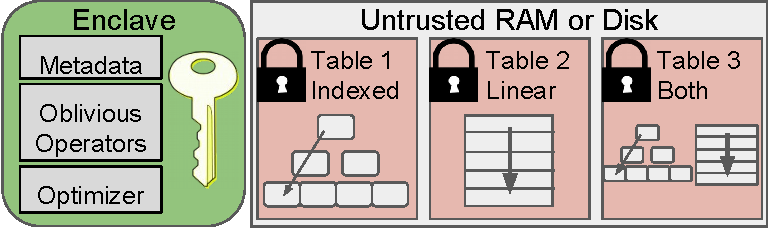
\includegraphics[width=\linewidth]{figure_revised.pdf}
\caption{\small \name/ provides an interface to a secure enclave with control over encrypted tables stored in untrusted memory. It stores tables either as an oblivious B+ tree index, a linear scan data structure or both to perform efficient oblivious queries.}
\label{arch}
\end{figure}
Figure~\ref{arch} shows an overview of the \name/ architecture. \name/ consists of a trusted code base inside an enclave that provides an interface for users to create, modify, and query tables. \name/ supports two \emph{storage methods} for each table: Linear and Indexed. It stores tables, encrypted, in unprotected memory and obliviously accesses them as needed by the various supported operators. Indexed tables consist of an ORAM with a B+ tree stored inside, whereas Linear tables scan the whole table on each query to ensure obliviousness.

  \name/ supports oblivious versions of the SQL operators \texttt{SELECT}, \texttt{INSERT}, \texttt{UPDATE}, \texttt{DELETE}, \texttt{GROUP BY} and \texttt{JOIN} as well as the aggregates \texttt{COUNT}, \texttt{SUM}, \texttt{MIN}, \texttt{MAX}, and \texttt{AVG}. Each operator is implemented for both Linear and Indexed tables. Finally, ObliDB includes a query optimizer that can choose the right operator plan for each query. For example, for selection queries, the optimizer first determines the size of the selection and then executes the best-performing \texttt{SELECT} algorithm for the data to be returned. Choices include algorithms that take advantage of the possibility of caching small results inside the enclave or quickly handling very large return sets by making a copy of the original table and returning it whole with the few missing rows obliviously erased.

\subsection{Limitations}
\name/ provides strong privacy guarantees with practical performance for a broad range of applications but was not designed as a distributed database system. Although this may render it unsuitable for certain high-performance settings, the vast majority of web applications only require a single-server database solution with the ability to efficiently handle diverse queries. This constitutes the target population \name/ hopes to entice as users in order to bring heightened privacy to everyday web users.

We note in this vein that however secure the properties of a database management system, an application interacting with it can leak additional information and must be secured as well. For example, if a web application using \name/ makes a second query to a database based on the results of a first query, observing the size of the response to the second query may leak additional information about the first query or its response. This direct, if unexpected, consequence of size leakage requires that application developers consider performance goals against the ramifications of such leakage in their design process.

\section{Background}\label{background}
In this section we give a basic overview of Intel SGX and ORAM, the primary tools used in \name/, providing only sufficient detail for the subsequent sections.

\subsection{Intel SGX}

SGX provides developers with the abstraction of a secure \textit{enclave} which can verifiably run a trusted code base (TCB) and protects its limited memory from a malicious or compromised OS \cite{CD16, SGXRef}. SGX handles the process of entering and exiting an enclave and hiding the activity of the enclave while non-enclave code runs, albeit imperfectly~\cite{LSG+16}. Enclave code invariably requires access to OS resources, so SGX provides an interface between the enclave and the OS based on \textit{OCALLs} and \textit{ECALLs}. OCALLs are calls made from inside the enclave to the OS, usually for procedures requiring resources managed by the OS, such as access to files on disk. ECALLs allow code outside the TCB to call the enclave to execute trusted code.

SGX proves that the code running in an enclave is an untampered version of the desired code through a mechanism named \textit{attestation}. Attestation involves an enclave providing a hash of its initial state which a client compares with the expected value of the hash and rejects if there is any evidence of a corrupted or altered program.

The most significant feature of SGX for our purposes concerns the protection of memory. SGX provides the developer with approximately 90MB of Enclave Page Cache (EPC), a memory region hidden from the OS and cleared whenever execution enters or exits an enclave. In this memory, the enclave can execute trusted code and keep secrets from a malicious OS who otherwise controls the machine executing the code.

\subsection{ORAM}
Oblivious RAM (ORAM), a cryptographic primitive first proposed by Goldreich and Ostrovsky~\cite{GO96}, hides access patterns to data in untrusted memory. In the traditional ORAM setting, a small trusted processor uses a larger memory over a bus where an adversary examines communications. Merely encrypting data over the bus still reveals the access patterns to the data being requested and can reveal private information about the data or the queries on it~\cite{IKK12}. ORAM goes further and shuffles the locations of blocks in memory so repeated accesses to the same block and other patterns are hidden from the adversary. ORAMs guarantee that any two sets of access patterns of the same length are indistinguishable from each other. ORAM security is formally defined as follows:
\begin{definition}[ORAM Security\cite{SDS+13}]
Let $\overrightarrow{y}:=\textbf{((op$_M$, a$_M$, data$_M$),...,(op$_1$, a$_1$, data$_1$))}$ denote a data request sequence of length $M$, where each \textbf{op$_i$} denotes a \textbf{read(a$_i$)} or a \textbf{write(a$_i$, data)} operation. Specifically, \textbf{a$_i$} denotes the identifier of the block being read or written, and \textbf{data$_i$} denotes the data being written. Index $1$ corresponds to the most recent load/store and index $M$ corresponds to the oldest load/store operation.

Let $A(\overrightarrow{y})$ denote the (possibly randomized) sequence of accesses to the untrusted storage given the sequence of data requests $\overrightarrow{y}$. An ORAM construction is said to be secure if:
\begin{enumerate}
\setlength\itemsep{0pt}
\item For any two data request sequences $\overrightarrow{y}$ and $\overrightarrow{z}$ of the the same length, their access patterns $A(\overrightarrow{y})$ and $A(\overrightarrow{z})$ are computationally indistinguishable by anyone but the client ORAM controller.

\item The ORAM construction is correct in the sense that it returns on input $\overrightarrow{y}$ data that is consistent with $\overrightarrow{y}$ with probability $\geq 1 - \textit{negl}(|\overrightarrow{y}|)$, i.e., the ORAM may fail with probability $\textit{negl}(|\overrightarrow{y}|)$.
\end{enumerate}
\end{definition}

The scope of ORAM's security guarantees create important consequences for oblivious data structures or algorithms built on it. ORAM only guarantees indistinguishability for access patterns of the same length, so algorithms using ORAM must always make the same number of memory accesses or risk leaking access patterns.

Although other, older schemes have recently received attention due their practical efficiency in certain practical parameter settings~\cite{ZWR+16}, the most efficient ORAM scheme known is the Path ORAM~\cite{SDS+13}. Path ORAM belongs to a family of schemes known as tree-based ORAMs, which operate by storing the blocks of the oblivious memory in a tree structure. Each block is associated with a leaf in the tree in a position map that guarantees the block will be found somewhere on the path to that leaf. An access to the ORAM involves reading a path down the tree from the root to the leaf corresponding to the desired block. After retrieving the desired block, a second pass is made on the same path where each block is re-encrypted with new randomness and the retrieved block is assigned a new leaf, remaining stored in a small ``stash'' if the path does not allow space for it to be written back on the path to its new assigned leaf. Although it is not always necessary in practice, the position map holding the assigned leaves for each block of the ORAM can be recursively stored in its own ORAM to reduce the trusted processor memory required by this scheme to a constant.

\section{\name/'s Storage Methods}\label{oblivData}
\name/ stores data at rest in two types of tables: Linear and Indexed. This section discusses each storage method and the security considerations involved in building algorithms for operators over them.

\name/ creates tables with an initial maximum capacity that can be increased later by copying to a new, larger table. Data can be represented by a Linear structure, an Indexed structure, or both in parallel, so as to take advantage of the properties of both table types. Since tables are stored in unprotected memory, \name/ independently encrypts and MACs every block of each data structure with a symmetric key generated inside the enclave. For both storage methods, it stores each row in one block of the corresponding data structure and reserves the first byte of each block as a flag to indicate whether that block contains a row or is empty.

\subsection{Linear Tables}
A Linear type table simply stores rows in a series of adjacent blocks with no additional mechanism to ensure obliviousness of memory accesses. This constitutes a ``trivial'' ORAM where every read or write to the table must involve accesses to every block of the structure in order to maintain obliviousness of access patterns. As such, operators acting on such a tables, as will be seen in Section~\ref{oblivOps}, involve a series of linear scans over the entire data structure. This data structure performs best with small tables, tables where operations will typically require returning large swaths of the table, or aggregates that involve reading most or all of the table regardless of the need for obliviousness. The challenge in designing algorithms for Linear tables lies in using the limited space of the enclave effectively to reduce the number of scans and data processing operations involved in each operator.

\subsection{Indexed Tables}
Indexed type tables make use of both an ORAM and a B+ tree in order to provide better performance without losing obliviousness for large data sets. The data structure consists of an ORAM that holds a B+ tree where the actual data of the table resides, with each node of the B+ tree corresponding to one block of the ORAM.

\noindent \textbf{New Tradeoffs}. The key insight in making this data structure efficient is that an ORAM underneath the B+ tree alters the usual performance tradeoffs inherent in B+ trees in unexpected ways. For example, in a typical B+ tree, the choice of maximum degree of nodes in the tree depends on a balance between achieving low depth overall and not having too many pointers to examine and update within a single node. ORAM upsets the balance on which this intuition relies by increasing the cost of following or updating pointers between nodes(each of which requires an ORAM lookup) to the point where many operations scanning child keys within a single node become almost free by comparison to following a pointer. As such, the degree of a node can become even bigger than usual well before the cost of operations within a node reaches parity with the cost of an ORAM operation. On the other hand, ORAM presents another constraint too: increasing the degree beyond a certain point requires ORAM blocks to become larger, reducing the performance of the underlying ORAM. We compromise by making the degree of our trees as high as possible without artificially inflating the size of ORAM blocks to accommodate pointers to additional children.

\noindent \textbf{Optimizing Worst-Case Performance}. Since we wish to preserve obliviousness in all queries, every B+ tree operation takes on its worst-case running time every time it runs, and the costs of usually uncommon splits and merges of nodes must be paid on every insertion or deletion to an Indexed table. To help mitigate the impact of this average case to worst case conversion incurred by obliviousness, \name/ reduces the number of writes needed to the ORAM for each B+ tree operation, operating on a lazy write-back principle where it does not write changes to the ORAM until the last possible moment.

Another example of where ORAM changes implementation decisions for oblivious B+ trees in surprising ways regards the case of parent pointers. A normal B+ tree may have pointers in each node to its parent as a low-cost solution to avoid a search down the tree to find a node's parent. This optimization even appears useful at first glance because we want to minimize the worst case time for each operation, and a parent pointer helps expedite the process of finding parents for the purposes of merging or splitting nodes, saving a handful of ORAM reads on every operation. However, each time a tree splits or merges a node, all the children of nodes involved need to have their parent pointers updated, a very slow process in the regime where every node requires an ORAM write to update.

\noindent \textbf{Memory Management}. The structure of a B+ tree changes dynamically as rows are added and removed from a database, so our B+ tree implementation must use some form of dynamic memory management and pointers between nodes in the tree. We implement equivalents of malloc, free and the pointer dereference operator for our ORAM. Our memory allocator consists of an array of flags that we set if the corresponding block is in use and unset if it is not. This increases the protected memory needed over the ORAM's position map by 20\% but does not represent a dramatic increase in memory requirements over the total space needed by \name/ for the position map, ORAM stash, and other elements of system state recording the names, sizes, and types of existing tables.

\subsection{Practical and Security Considerations}

\begin{figure}
\small
\begin{tabular}{r|ccc}
Method&Linear&Index&Combined\\\hline
Space &$N$&\textasciitilde$4N$&\textasciitilde$5N$\\
Point Read&$O(N)$&$O(log^2N)$&$O(log^2N)$\\
Large Read&$O(N)$&$O(NlogN)$&$O(N)$\\
Insertion&$O(1)$&$O(polylogN)$&$O(polylogN)$\\
Deletion&$O(N)$&$O(polylogN)$&O(N)\\
\end{tabular}
\caption{\small Asymptotic performance of each storage method.}
\label{asymTables}
\end{figure}

\noindent \textbf{Choosing Storage Methods}. \name/ currently has system administrators decide which storage format to use for each table, a decision easily made based on the kinds of queries that are expected to be run on the data. Indexed tables perform best on small reads that access one or a few rows of a table, whereas queries which expect to return large segments of a table should use Linear tables. Using both types of table, while incurring the cost of both for insertions and deletions, proves effective when queries of diverse selectivities must run on the same data. Figure~\ref{asymTables} compares the asymptotic operations of standard read, insertion, and deletion operations on each table type.

 \noindent \textbf{Obliviousness}. Although the security properties of ORAM guarantee that two access transcripts of the same length will be indistinguishable from each other, designers of oblivious algorithms for operators over Indexed tables must ensure that the total number of accesses or the timing gaps between accesses do not leak any private data. For example, the property of the B+ tree that all data resides in the leaves of the tree, always at the same depth, means that any search in the tree will make the same number of accesses to intermediate nodes before finding the desired data. Using a different data structure that does not exhibit such a property would compromise the obliviousness of our operators on Indexed tables. On the other hand, standard insertion and deletion operations for B+ trees leak information about the internal structure of the tree because they involve splitting and merging nodes when they reach fixed threshold numbers of children. Even in a Linear table, satisfying a \texttt{SELECT} query via a straightforward scan that copies each row matching the given criteria into an output table does not provide obliviousness despite touching every row in the table. Such an approach still leaks which rows we include in the output because an attacker can watch the output table and take note of which points in the scan coincide with growth in the output table. We address considerations in ensuring obliviousness for each operator in Section~\ref{oblivOps}.

 \noindent \textbf{Data Integrity}.
Although encryption and oblivious data structures/algorithms ensure the privacy of data in \name/, additional protections make certain that an attacker does not tamper with data. Such tampering could take the form of editing within rows of a table, addition/removal of rows, shuffling the contents of a table, or rollbacks to an old system state. \name/ protects against such attacks and reports any attempt to tamper with data.

\name/ MACs and encrypts every block of data stored outside the enclave, preventing the OS from modifying rows or adding new rows to tables. This leaves the possibility of duplicating/removing rows, shuffling rows, or rolling back the system state. Included in each block of MACed data is a record of which row the block contains and its current ``revision number,'' a copy of which \name/ also stores inside the enclave. Any attempt to duplicate, shuffle, or remove rows within a data structure will be caught when an operator discovers that the row number of data it has requested does not exist or does not correspond to that which it has received. Spoofing a fake revision number requires either breaking the security of the MACs used or breaking the security of the enclave to modify the stored copy, neither of which lies within the power of an attacker in our model. Rollbacks of system state are caught when the revision numbers of rows in a table do not match the last revision numbers for those rows recorded in the enclave. These lightweight protections suffice to discover and block any malicious tampering of data in \name/.

\section{Oblivious Operators}\label{oblivOps}
In this section we describe the various oblivious operator algorithms used in \name/. \name/ provides support for a large subset of SQL, including insertions, updates, deletions, joins, aggregates (count, sum, max, min, average), groupings, and selection with conditions composed of arbitrary logical combinations of equality or range queries. Moreover, depending on known information about the size of a response to a query, \name/ can choose which algorithm to use in order to maximize performance in each situation. We will begin by discussing algorithms for Linear tables and then discuss the modifications or entirely different solutions used for Indexed tables. Each operation will be accompanied by a security argument.

The following notation will be used in subsequent paragraphs: the table being returned will be referred to as $R$, and the table being selected from will be referred to as $T$. The number of rows in $R$ is represented by $r$, the number of rows in $T$ is $N$. $r'$ and $N'$ represent the number of blocks in the data structures holding $R$ and $T$, respectively.

\subsection{Linear Tables}
  \noindent \textbf{Insert, Update, Delete}.
Insertions, updates, and deletions for Linear tables involve one pass over the table, during which any unaffected block receives a dummy write (overwriting a row with the data it already held, re-encrypted) and affected blocks are written to as follows:

\emph{Insertion:} \name/ offers two options for insertions in Linear tables. First, it can conduct a linear scan, making dummy writes on each row except the first unused block, where it makes a real write. In tables with few deletions, a fast insertion algorithm recalls the last row where an insert occurred and inserts directly into the next row.

\emph{Deletion:} any row matching the deletion criteria will be marked as unused and overwritten with dummy data. Deletions and updates support arbitrary conditions, similar to selections, so any logical combination of conditions on equality or inequality of entries in a row is acceptable.

\emph{Update:} any row matching the update criteria will have its contents updated instead of a dummy write.


All of the above operations, with the exception of fast insertion, leak nothing about the parameters to the query being executed or the data being operated on except the sizes of the data structures involved because they consist of one linear scan over a table where each encrypted block is read and then written with a fresh encryption. Fast insertion also leaks no additional information beyond the sizes of tables because the access pattern of the insert does not depend at all on the content of the data except on the number of insertions made, which our adversary can already learn by observing the sizes of tables over time.

  \noindent \textbf{Select}.
Our Select algorithm begins by scanning once over the desired table and counting the number of rows that are to be selected. This step leaks only the size of the table $T$. Then, based on the size of the output set and whether the selected rows form one continuous block in the table or not, it executes one of several strategies:

\textit{Na\"ive}: included as a baseline for comparison, the na\"ive oblivious algorithm mirrors a straightforward translation of a non-oblivious \texttt{SELECT} to an oblivious one via an ORAM. After examining each row, it executes an ORAM operation. If the examined row is to be included in the output, it makes a write. If not, it makes a dummy read (reading an arbitrary block). After completing the scan of the input table, it copies the ORAM to a Linear table which it returns.

Our techniques to improve upon this baseline consist of finding the right balance between using data structures inside the enclave to remove the need for an ORAM and making multiple fast passes over data. These ideas constitute the guiding principle in designing our remaining \texttt{SELECT} algorithms and choosing between them.

\textit{Continuous}: Should the rows selected form one continuous section of the data stored in the table, a common special case, \name/ employs a different strategy that requires only one additional pass over the table. First, it creates table $R$ with $r$ rows. Then, for the $i$th row in table $T$, if that row should be in the output, it writes the row to position $i\bmod r$ of $R$. If not, it makes a dummy write. Since the rows that need to be included in $R$ make up one continuous segment of $T$, this procedure results in exactly the selected rows appearing in $R$.

In addition to the sizes of tables $T$ and $R$, the fact that \name/ chooses this algorithm over one of the other options leaks the fact that the result set is drawn from a continuous set of rows in the table. Users concerned about this additional leakage could disable this option and use one of the other options with no reduction in supported functionality. The execution of the algorithm itself is oblivious, however, because the memory access pattern is fixed: at each step, the algorithm reads the next row of $T$ and then writes to the next row of $R$.

\textit{Small}: In the case where $r$ is small, that is, where all the rows of table $R$ only require a few times the space available in the enclave, a selection strategy that makes multiple fast passes over the data proves effective. We take multiple passes over table $T$, each time storing any selected rows into a buffer in the enclave and keeping track of the index of the last checked row. Each time the buffer fills, its contents  are written to $R$ after that pass over $T$. Although this strategy could result in a number of passes linear in the size of $R$, it proves effective for small $r$, as demonstrated in Section~\ref{eval}.

This algorithm leaks only the sizes of tables $T$ and $R$ because every pass over the data consists only of reads to each row of the table and the number of passes reveals only how many times the output set will fill the enclave, a number that can be calculated from the size of $R$, which we reveal anyway.

\textit{Large}: If table $R$ contains almost every row of table $T$, we create $R$ as a copy of $T$ and then make one pass over $R$ where each unselected row is marked unused and each selected row receives a dummy write.

The copy operation reveals no additional information about $T$ or $R$ because it could be carried out by a malicious OS with no input from the enclave or a user. The process of clearing unselected rows involves a read followed by a write to each block of the table, so it also reveals no information beyond the size of $T$. This algorithm, in fact, does not even reveal the size of the output set $R$ because we pad the data structure to the size of~$T$.

\textit{Hash}: In the case that none of the preceding special-case algorithms apply, \name/ uses the following generalization of the continuous strategy. We wish to apply the technique used for continuous data on data that may be arbitrarily spread throughout $T$, not just in one continuous block. Our approach is to resort to a hashing-based solution. For the $i$th row in $T$, if the row is to be included in the output, we write the content of the row to the $h(i)$th position in $R$, for some hash function $h$.

The algorithm as stated above does not exactly represent how \name/ works because we need a few changes in order to ensure, first, that we properly handle hash collisions to ensure correctness, and, second, that we maintain obliviousness in handling collisions. In order to maintain obliviousness, every real or dummy write to $R$ must involve the same number of accesses to memory. This means that if any write resolves in a collision, every write must make as many memory accesses as in the case of a collision. Following the guidance of Azar et al~\cite{ABKU99}, we use double hashing and have a fixed-depth list of 5 slots for each position in $R$. This means that for each block in $T$, there will be 10 accesses to $R$, 5 for each of the two hash functions.

The modifications above ensure that data access patterns are fixed regardless of the data in the table and which rows the query selects. Since the hash is taken over the index of the row in the data structure and not over the actual contents of a row, information about the data itself cannot be leaked by access patterns when rows are written to $R$. As such, only the sizes of $T$ and $R$ leak. The selection strategy also leaks, but this information can be deduced just from knowledge of the sizes of $T$ and $R$ and therefore leaks no additional information.

  \noindent \textbf{Aggregates \& Group By}.
A baseline solution to aggregation queries performs very poorly, but we can compute aggregates far faster than selection and only require one oblivious pass over a Linear table to do so.  An aggregate over a whole table or some selected subset of a table requires only one pass over the whole table where we calculate the aggregate cumulatively based on the data in each row. A na\"ive approach uses an ORAM to keep track of the aggregate and needs to access it for every row, causing an unnecessary slowdown. We achieve better performance by keeping the aggregate statistic inside the enclave and avoiding the ORAM overhead. Since the memory access pattern of this operation always involves sequential reads of each block in the data structure, nothing leaks from this operation beyond the size of table~$T$.

We handle groupings similarly to aggregates without groupings, except we keep an array inside the enclave that keeps track of the aggregate for each group where a na\"ive solution would check an entire array via oram for each row of table $T$. The method for determining which group each row belongs to is handled differently for low and high-cardinality aggregation:

\textit{Low-Cardinality}: In the low-cardinality setting, we make a linear scan over known groups in order to check for a match. If we find no match, we create a new group.

\textit{High-Cardinality}: Linearly scanning over all known groups becomes prohibitively expensive as the number of groups becomes larger, so high-cardinality groupings employ a hash table where each group's value is hashed and inserted into a hash table held in the enclave. Each row scanned is hashed and checked against the table. If there is a match, then the row under examination corresponds to a known group referenced in the table, and if not, then the current row is added as a new group.


  \noindent \textbf{Join}.
We implement the join functionality for Linear tables as a variant of the standard hash join algorithm~\cite{EN10}. We refer to the two tables being joined as $T_1$ and $T_2$. The Join proceeds by making a hash table out of as many rows of $T_1$ as will fit in the enclave and then hashing the variable to be joined from each row of $T_2$ to check for matches. This process repeats until reaching the end of $T_1$ . After each check, a row is written to the next block of an output linear table. If there is a match, the joined row is written. If not, a dummy row is written to the table at that position. This algorithm reveals the sizes of the tables $T_1$ and $T_2$, but not the size of the output table, which is padded to a parameter representing the maximum possible size by dummy rows (which can be set to less than $|T_1|*|T_2|$ if desired). Since each comparison between the two tables results in one write to the output structure regardless of the results of the comparison, the memory access pattern of this algorithm is oblivious.

\subsection{Indexed Tables}
Operations for Indexed tables largely behave similarly to those for Linear tables, except all the operations take place over the ORAM and B+ tree data structure described in Section~\ref{oblivData}. The important difference between the two lies in the fact that the index can restrict a search to a particular relevant area of a table without having to scan every row to maintain obliviousness. The use of an index, however, comes with some security ramifications. In the case that the block of rows accessed by a query are a continuous set beginning and ending with a specified value of the index column, no additional information leaks because knowledge of the size of the portion of the table scanned is equivalent to knowledge of the size of the query output. On the other hand, if the rows returned by a query are not continuous, the leakage also includes the size of the segment of the database scanned in the index. For example, supposing that there is one student named Fred in a table of students indexed by student IDs, the query \texttt{SELECT * FROM students WHERE NAME = ``Fred'' AND ID > 50 and ID < 60} leaks not only that the size of the result set is 1 but also that 9 rows were scanned in the execution of the query. We consider this leakage to be included in the sizes of intermediate tables, as a query plan that selects a noncontinuous segment from an Indexed table is equivalent to one which selects a continuous segment from an Indexed table and then selects a noncontinuous segment from the returned table. This leakage can, of course, be hidden by padding.

  \noindent \textbf{Insert, Update, Delete}.
  Insertions and Deletions for Indexed tables pad the number of operations made on the underlying ORAM so no information can be leaked about the internal structure of the B+ tree. As discussed in Section~\ref{oblivData}, this means every B+ tree operation has worst-case running time and that design decisions involved in constructing the trees and operations on them differ from the traditional setting without ORAM. Updates on segments of an Indexed table behave similarly to Linear tables.

  \noindent \textbf{Select, Aggregates, \& Group By}.
  Indexed tables make use of the same selection, aggregation, and grouping algorithms as linear tables, with the major difference being the use of the index to find the correct part of a table to scan. The Large strategy for selection does not apply to Indexed tables because the strategy of copying the whole table is not as applicable where a query aims at a small fraction of the table and the data are not stored in consecutive blocks but across multiple nested tree-based data structures.

  \noindent \textbf{Join}.
  Since the rows of an Indexed table are always sorted by the index column in the leaves of the B+ tree, it is possible to efficiently sort-merge join two tables with the same index~\cite{EN10}. Tables $T_1$ and $T_2$ are scanned at the same time, and any matching rows are placed in an output ORAM, just as for Linear tables. More specifically, at each step, the next row of each of $T_1$ and $T_2$ is read. If the rows match, the pointer on the right table advances and there is a write to the ORAM, and if they do not match, a dummy write takes place and the pointer on the table with the lesser value advances. This process proceeds until pointers reach the end of both tables. Obliviousness holds because each step of the algorithm consists of exactly one read to each of $T_1$ and $T_2$ and one write to an ORAM, and the total number of steps is only a function of the sizes of the three data structures involved.

\subsection{Complexity}
Prior systems that implement oblivious operators include Opaque~\cite{ZDB+17}, Cipherbase~\cite{cipherbase}, and the Oblivious Query Processing algorithms of Arasu and Kaushik~\cite{AK14}. All three works focus on oblivious algorithms for analytic queries and only propose algorithms that involve scans over entire tables. The approach to this kind of operator typically involves a combination of oblivious sorts and filters. In contrast, our work uses new ideas to achieve similar functionalities for both Linear and Indexed tables, providing support for a broader set of general database use cases. Whereas sort and filter based approaches always have complexity $O(N)$ or $O(N\textit{log}N)$ in the size $N$ of a table, \name/'s solutions range in complexity from $O(1)$ to $O(N^2)$, but our optimizer picks the algorithms it expects will perform best in practice regardless of asymptotics.

\section{Implementation}\label{imp}
Our implementation of \name/ includes the linear scan and oblivious B+ index from Section~\ref{oblivData} as well as the oblivious operator algorithms described in Section~\ref{oblivOps}. It consists of over 14,000 lines of code of which approximately 10,000 are new and builds upon the Remote Attestation sample code provided with the SGX SDK ~\cite{SGXRef} and the B+ tree implementation of~\cite{BPlus}, the latter of which was heavily edited in order to support our ORAM memory allocator. We used the libraries made available by the SGX SDK for encryption, MACs, and hashing. We will make \name/ open source and publicly available online.

We tuned ObliDB's parameters for the protected memory space made available by SGX. We chose a nonrecursive PATH ORAM~\cite{SDS+13} as our choice of ORAM scheme. The nonrecursive ORAM can fit up to about 15 million rows before needing a second layer of recursion in order to fit the position map in an SGX enclave, so \name/ can handle realistic data sets without any need for a recursive ORAM. That said, there is no reason why \name/ cannot be modified to make use of recursive ORAM at a modest performance penalty for Indexed tables. Moreover, the \name/ implementation allows for easy swapping of ORAM schemes through a common interface, so our choice of ORAM can easily be replaced, say, to optimize the ORAM scheme used to fit the data as in~\cite{ZWR+16}.

\section{Evaluation}\label{eval}
\begin{figure}
\small
\centering
\begin{tabular}{llp{3.5cm}}
\textbf{Table Name} & \textbf{Rows} & \textbf{Notes} \\\hline\rule{0pt}{2ex}
CFPB & 107,000 & Customer complaints to the US Consumer Financial Protection Bureau~\cite{CFPB}.\\
USERVISITS & 350,000 & Server logs for many sites. Part of the Big Data Benchmark data set~\cite{BDB}.\\
RANKINGS & 360,000 & URLs, PageRanks, and average visit durations for many sites. Part of the Big Data Benchmark data set~\cite{BDB}.\\
\end{tabular}
\caption{\small Real data used in our evaluation and comparisons.}
\label{tabletable}
\end{figure}

\begin{figure*}
\small
\centering
\begin{tabularx}{\textwidth}{p{1.9cm} X l l l}
 \textbf{Data Set}& \textbf{Query}& \textbf{\name/} & \textbf{Baseline} & \textbf{Speedup}\\ \hline\rule{0pt}{2ex}
 &\multicolumn{2}{c}{\textbf{Linear Selection}}\\\rule{0pt}{2ex}
CFPB & \footnotesize\texttt{SELECT * FROM CFPB WHERE Date\_Received$=$2013-05-14}& 1.192s & 34.79s & 29.2$\times$\\\rule{0pt}{2ex}
RANKINGS & \footnotesize\texttt{SELECT pageURL, pageRank FROM RANKINGS WHERE pageRank > 1000 }& 2.434s & 46.33s& 19.0$\times$ \\\rule{0pt}{2ex}
&\multicolumn{2}{c}{\textbf{Index Selection}}\\\rule{0pt}{2ex}
CFPB & \footnotesize\texttt{SELECT * FROM CFPB WHERE Date\_Received$=$2013-05-14} & 0.472s & 0.678s & 1.4$\times$\\\rule{0pt}{2ex}
CFPB & \footnotesize\texttt{SELECT * FROM CFPB WHERE Date\_Received$=$2017-08-17} (point query) & 0.0027s & 0.0033s & 1.5$\times$\\\rule{0pt}{2ex}
RANKINGS & \footnotesize\texttt{SELECT pageURL, pageRank FROM RANKINGS WHERE pageRank > 1000 }& 0.082s & 0.107s& 1.3$\times$ \\\rule{0pt}{2ex}
&\multicolumn{2}{c}{\textbf{Index Insertion/Deletion}}\\\rule{0pt}{2ex}
CFPB & \footnotesize\texttt{INSERT INTO CFPB (Complaint\_id, Product, Issue, Date\_received, Company, Timely\_response, Consumer\_disputed) VALUES (4242, "Credit Card", "Rewards", 2017-09-01, "Bank of America", "Yes", "No")}& 0.011s& 0.708s& 64.4$\times$ \\\rule{0pt}{2ex}
\ignore{CFPB & \footnotesize\texttt{DELETE FROM CFPB WHERE Bank="Bank of America" WHERE Date\_Received$=$2013-05-14 LIMIT 1}& 0.224s& 0.451s& 2.0$\times$ \\\rule{0pt}{2ex}}
CFPB & \footnotesize\texttt{DELETE FROM CFPB WHERE Bank="Bank of America" AND Date\_Received$=$2017-08-17} (point query)& 0.015s& 0.220s& 15.0$\times$ \\\rule{0pt}{2ex}
&\multicolumn{2}{c}{\textbf{Aggregates and Joins}}\\\rule{0pt}{2ex}
CFPB & \footnotesize\texttt{SELECT COUNT(*) FROM CFPB WHERE (Product="Credit card" OR Product="Mortgage") AND Timely\_Response="No" GROUP BY Bank}& 0.595s & 110.3s & 185.4$\times$\\\rule{0pt}{2ex}
USERVISITS & \footnotesize\texttt{SELECT SUBSTR(sourceIP, 1, 8), SUM(adRevenue) FROM USERVISITS GROUP BY SUBSTR(sourceIP, 1, 8)}& 3.042s &$>$1000s & $>$328.7$\times$\\\rule{0pt}{2ex}
USERVISITS, RANKINGS & \footnotesize\texttt{SELECT sourceIP, totalRevenue, avgPageRank
FROM
  (SELECT sourceIP,
          AVG(pageRank) as avgPageRank,
          SUM(adRevenue) as totalRevenue
    FROM Rankings AS R, UserVisits AS UV
    WHERE R.pageURL = UV.destURL
       AND UV.visitDate BETWEEN Date(`1980-01-01') AND Date(`1980-04-01')
    GROUP BY UV.sourceIP)
  ORDER BY totalRevenue DESC LIMIT 1} & 12.774s & $>$1000s& $>$78.3$\times$\\
\end{tabularx}
\caption{\small Comparison of \name/ and a baseline where a na\"ive oblivious database implementation directly ports non-oblivious algorithms to their oblivious counterparts via ORAM. \name/ outperforms the baseline on all queries. Our aggregate and join queries were run over Linear tables because they involve reading most or all rows of the relevant tables.}
\label{figQueries}
\end{figure*}
In this section we evaluate \name/ on tables of up to 1.4 million rows and measure its performance against a baseline implementation that na\"ively modifies a database to use ORAM as well as existing private database systems. A summary of real-world data sets used in our experiments appears in Figure~\ref{tabletable}. We also measure the overhead of \name/'s padding mode and  demonstrate the effectiveness of \name/'s query optimizer as well as the efficacy of Linear and Indexed tables in different situations through a series of microbenchmarks. We evaluated \name/ on a desktop computer with an Intel Core i7-6700 CPU @3.4GHz and 8GB of RAM running Ubuntu 16.04.2 and the SGX Linux SDK version 1.9~\cite{SGXRef}.

We find that \name/ dramatically outperforms a baseline implementation and can leverage its indexes to achieve order of magnitude performance improvements over previous private database systems. In particular, \name/ matches Opaque~\cite{ZDB+17} for scan-based queries but can outperform it by 18.8x when it uses an index. \name/ also performs 22.6-24.6$\times$ faster than Sophos~\cite{Bost16}, a recent index-based searchable encryption scheme.

\subsection{Comparison to Na\"ive ORAM Baseline}

\name/ outperforms a na\"ive baseline ORAM implementation (i.e. what could be achieved with a generic tool for converting legacy applications to use ORAM) by as much as two orders of magnitude.  Since a direct translation of the memory accesses of a non-oblivious data structure to an ORAM does not guarantee obliviousness (e.g., if different operations make different amounts of ORAM accesses), we modified several standard database data structures and algorithms as little as possible to achieve an oblivious version for our baseline, always erring on the side of stronger performance. Our baseline uses the same data structure as \name/ for Linear tables but uses a na\"ive B+ tree implementation that does not take advantage of the ORAM-related optimizations discussed in Section~\ref{oblivData}. The baseline also uses the na\"ive varieties of operators as described in Section~\ref{oblivOps}.

Figure~\ref{figQueries} compares \name/ to our na\"ive ORAM baseline. \name/ achieves up to 29$\times$ speedup for \texttt{SELECT} queries and over 328$\times$ speedup for aggregates. For comparison to an insecure system, a point selection query in \name/ performs only 7.9$\times$ slower than in mysql over a table stored in memory. \texttt{SELECT} queries over Linear tables enjoy much larger speedup over the baseline than queries over Indexed tables because an oblivious B+ tree lookup takes most of time in the indexed \texttt{SELECT} queries. We used the same algorithm for this lookup in both the baseline and actual implementations. We did this because a na\"ive application of ORAM to a B+ tree does not yield an oblivious B+ tree, as described in Section~\ref{oblivData}.

The largest speedups over the baseline appear in aggregation queries, where \name/ gains two orders of magnitude in performance. This arises from the need to hide data structures that keep statistics for each group without revealing when a row does not match with any known groups and needs to begin its own new group. The possibility of this occurrence necessitates, in the na\"ive algorithm, an access to each group's data for each row. With the system-wide maximum number of groups set to the hundreds of thousands, such a query cannot complete within a reasonable time frame and may take well over the 1,000 seconds at which we cut off our experiments. The aggregation over the CFPB table completes in a shorter period of time because we used our prior knowledge of the number of banks to set the maximum number of groups to a lower threshold (200, in this case).

\begin{figure*}
\begin{minipage}{.64\textwidth}
\small
\centering
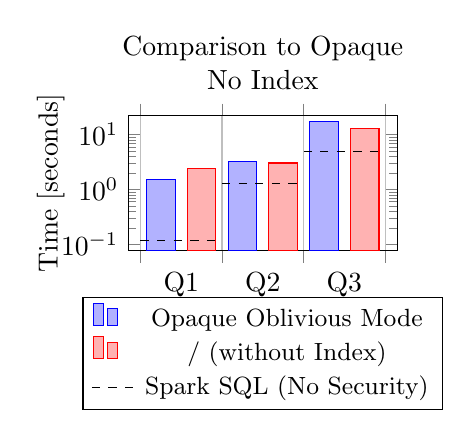
\begin{tikzpicture}
\centering
\begin{semilogyaxis}[
	log origin = infty,
	width=5cm,height=3.3cm,
	y label style={at={(axis description cs:-0.2,.5)},anchor=south},
	ytick={.1,1,10},
	ymin=.1,
	ylabel={Time [seconds]},
    title style={align=center},title={Comparison to Opaque\\No Index},
	symbolic x coords={Q1, Q2, Q3, 4},
	x tick label style={
		/pgf/number format/1000 sep=},
	%%ylabel=Time (seconds),
	enlargelimits=0.05,
	legend style={at={(0.5,-0.34)},
	legend entries={\small Opaque Oblivious Mode, \small \name/ (without Index), \small Spark SQL (No Security)},
	anchor=north,legend columns=1},
	ybar interval=.7,
    ]
%\addplot %baseline
%	coordinates {(BDB Q1, 54.18978) (BDB Q2, 205.78637) (BDB Q3, 131.29887) (4,1)};
\addplot %opaque obliv
	coordinates {(Q1,1.54659) (Q2,3.210607) (Q3,17.26355) (4, 1)};
\addplot %us
	coordinates {(Q1,2.434) (Q2, 3.0422) (Q3,12.774) (4,1)};
%\addplot %spark sql
%	coordinates {(BDB Q1,.1615) (BDB Q2,1.9757) (BDB Q3,7.2477) (4,1)};
    %\legend{Opaque Oblivious Mode,\name/, Spark SQL (No Security)}

\addlegendimage{line legend,black,sharp plot,dashed}
\coordinate (A) at (axis cs:Q1,.11755);
\coordinate (B) at (axis cs:Q2,.11755);
\coordinate (C) at (axis cs:Q2,1.2848);
\coordinate (D) at (axis cs:Q3,1.2848);
\coordinate (E) at (axis cs:Q3,4.8357);
\coordinate (F) at (axis cs:4,4.8357);

\draw [black,sharp plot,dashed] (A) -- (B);
\draw [black,sharp plot,dashed] (C) -- (D);
\draw [black,sharp plot,dashed] (E) -- (F);

\end{semilogyaxis}
\end{tikzpicture}
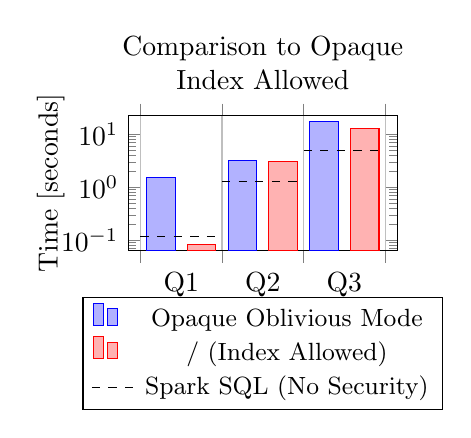
\begin{tikzpicture}
\centering
\begin{semilogyaxis}[
	log origin = infty,
	width=5cm, height=3.3cm,
	y label style={at={(axis description cs:-0.2,.5)},anchor=south},
	ylabel={Time [seconds]},
    title style={align=center},title={Comparison to Opaque\\Index Allowed},
	symbolic x coords={Q1,  Q2,  Q3, 4},
	x tick label style={
		/pgf/number format/1000 sep=},
	%%ylabel=Time (seconds),
	enlargelimits=0.05,
	legend style={at={(0.5,-0.34)},
		legend entries={\small Opaque Oblivious Mode, \small \name/ (Index Allowed), \small Spark SQL (No Security), \name/},
	anchor=north,legend columns=1},
	ybar interval=.7,
    ]
%\addplot %baseline
%	coordinates {( Q1, 54.18978) ( Q2, 205.78637) ( Q3, 131.29887) (4,1)};
\addplot %opaque obliv
	coordinates {(Q1,1.54659) (Q2,3.210607) (Q3,17.26355) (4, 1)};
\addplot %us
	coordinates {(Q1,.0824) (Q2, 3.0422) (Q3,12.774) (4,1)};
%\addplot %spark sql
%	coordinates {(Q1,.1615) (Q2,1.9757) (Q3,7.2477) (4,1)};
    %\legend{Opaque Oblivious Mode,\name/, Spark SQL (No Security)}

    \addlegendimage{line legend,black,sharp plot,dashed}
\coordinate (A) at (axis cs: Q1,.11755);
\coordinate (B) at (axis cs: Q2,.11755);
\coordinate (C) at (axis cs: Q2,1.2848);
\coordinate (D) at (axis cs: Q3,1.2848);
\coordinate (E) at (axis cs: Q3,4.8357);
\coordinate (F) at (axis cs:4,4.8357);
%\coordinate (G) at (60,-2);
%\coordinate (H) at (90,-2);
%\coordinate (I) at (60,-4);
%\coordinate (J) at (90,-4);

\draw [black,sharp plot,dashed] (A) -- (B);
\draw [black,sharp plot,dashed] (C) -- (D);
\draw [black,sharp plot,dashed] (E) -- (F);
%\draw [red,sharp plot,solid] (G) -- (H);
\end{semilogyaxis}
\end{tikzpicture}
\end{minipage}\hspace{.2cm}
\begin{minipage}{.32\textwidth}
\small
\centering
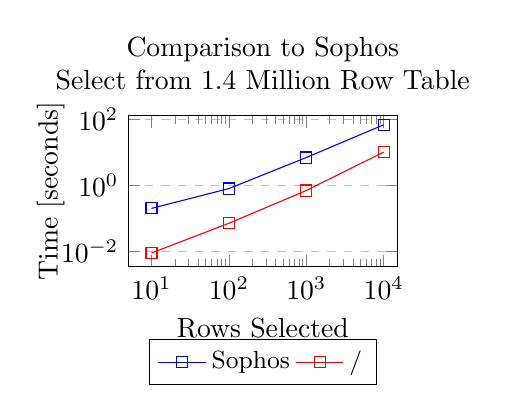
\begin{tikzpicture}
\begin{loglogaxis}[
    title style={align=center}, title={Comparison to Sophos\\Select from 1.4 Million Row Table},
    width=5cm, height=3.5cm,
    xlabel={Rows Selected},
	y label style={at={(axis description cs:-0.2,.5)},anchor=south},
	ylabel={Time [seconds]},
    xmin=5, xmax=15000,
    ymin=0, ymax=130,
    xtick={10,100,1000,10000},
    %ytick={0,10,20,30,40,50,60,70},
    legend pos=south east,
    ymajorgrids=true,
    grid style=dashed,
    	legend style={at={(0.5,-.48)},
		legend entries={\small Sophos, \small \name/},
	anchor=north,legend columns=2},
    ]
    \addplot[
    color=blue,
    mark=square,
    ]
    coordinates {
    (10,.2)(100,.8)(1000,7)(10000,69)
    };
    \addplot[
    color=red,
    mark=square,
    ]
    coordinates {
    (10,.00885)(100,.07083)(1000,.69767)(10000,10.24335)
    };
    %\legend{\scriptsize Sophos, \scriptsize \name/}
\end{loglogaxis}
\end{tikzpicture}\vspace{.3cm}
\end{minipage}
\begin{minipage}{.64\textwidth}
\caption{\small \name/ outperforms Opaque Oblivious~\cite{ZDB+17} by 1.1-18.8$\times$ and never runs more than 2.6$\times$ slower than Spark SQL~\cite{SparkSQL} on Queries Q1-Q3 of the Big Data Benchmark~\cite{BDB}. Even without use of an index, \name/ performs comparably to Opaque Oblivious.}
\label{figOpaque}
\end{minipage}\hspace{.2cm}
\begin{minipage}{.32\textwidth}
\caption{\small Comparison to Sophos SSE scheme\cite{Bost16}. \name/ always outperforms Sophos by at least 22.6$\times$. Unlike \name/, Sophos leaks access patterns to data.}
\label{figSophos}
\end{minipage}
\end{figure*}
\subsection{Comparison to Opaque}

Figure~\ref{figOpaque} compares \name/ with Opaque's oblivious mode~\cite{ZDB+17} and Spark SQL~\cite{SparkSQL} on queries 1-3 of the Big Data Benchmark~\cite{BDB} on tables of 360,000 and 350,000 rows. We omit the benchmark's query 4 as neither \name/ nor Opaque support the external scripts it requires. Opaque also uses an SGX enclave and can be configured in either ``encryption'' mode, which leaks access patterns but offers performance close to Spark SQL and ``oblivious'' mode that hides access patterns to data by making sure to fit sensitive memory accesses inside the trusted enclave memory, achieving a security level similar to ours, albeit by different means. Spark SQL provides no security guarantees. Both Opaque and Spark SQL run in single node configuration on our device.

\name/, when allowed to use indexes, outperforms Opaque on all three BDB queries, ranging from 1.1$\times$ speedup on query 2 to 18.8$\times$ speedup on query 1. The strong performance of \name/ compared to Opaque and Spark SQL on query 1 is due to \name/'s oblivious index, which allows it to only examine a fraction of the table whereas Opaque and Spark SQL, which primarily handle analytic workloads, scan the entire table. Indexes do not provide a speedup on queries 2 and 3 because those queries require scanning larger segments of the input tables. Even without using an index to speed up query 1, \name/ performs comparably to Opaque. Moreover, for queries 2 and 3, although \name/ is slower than Spark SQL, it is only 2.4$\times$ slower on query 2 and 2.6$\times$ slower on query 3, putting \name/ safely in the realm of tools with practical performance for real applications.
\begin{figure*}
\small
\centering
\begin{tabular}{@{}l@{}l@{}l}
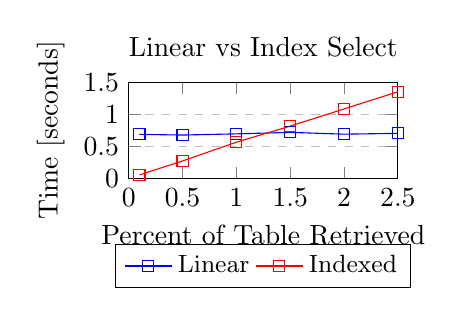
\begin{tikzpicture}
\begin{axis}[
    title={Linear vs Index Select},
    	width=5cm, height=2.8cm,
    xlabel={Percent of Table Retrieved},
    ylabel={Time [seconds]},
    xmin=0, xmax=2.5,
    ymin=0, ymax=1.5,
    xtick={0,.5,1,1.5,2, 2.5},
    %ytick={0,.25,.5,.75,1},
	legend style={at={(0.5,-0.68)},
	anchor=north,legend columns=-1},
    ymajorgrids=true,
    grid style=dashed,
    ]
    \addplot[
    color=blue,
    mark=square,
    ]
    coordinates {
    (.1,.6886)(.5,.6784)(1,.6968)(1.5,.7203)(2,.6922)(2.5,.7049)
    };
    \addplot[
    color=red,
    mark=square,
    ]
    coordinates {
    (.1,.0556)(.5,.2732)(1,.5666)(1.5,.8177)(2,1.0866)(2.5,1.3544)
    };
    \legend{\small Linear, \small Indexed}
\end{axis}
\end{tikzpicture}

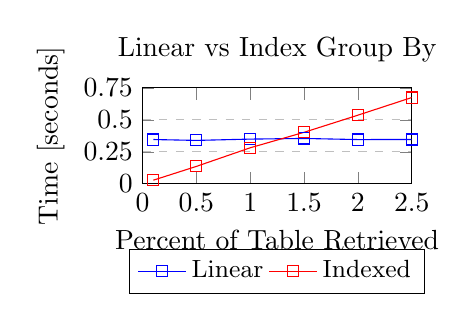
\begin{tikzpicture}
\begin{axis}[
    title={Linear vs Index Group By},
        ylabel={Time [seconds]},
        	width=5cm,height=2.8cm,
    xlabel={Percent of Table Retrieved},
    xmin=0, xmax=2.5,
    ymin=0, ymax=.75,
    xtick={0,.5,1,1.5,2, 2.5},
    ytick={0,.25,.5,.75},
	legend style={at={(0.5,-0.68)},
	anchor=north,legend columns=-1},
    ymajorgrids=true,
    grid style=dashed,
    ]
    \addplot[
    color=blue,
    mark=square,
    ]
    coordinates {
    (.1,.3462)(.5,.3393)(1,.3495)(1.5,.3546)(2,.3458)(2.5,.3465)
    };
    \addplot[
    color=red,
    mark=square,
    ]
    coordinates {
    (.1,.0282)(.5,.1361)(1,.2816)(1.5,.4025)(2,.5365)(2.5,.6744)
    };
    \legend{\small Linear, \small Indexed}
\end{axis}
\end{tikzpicture}
&
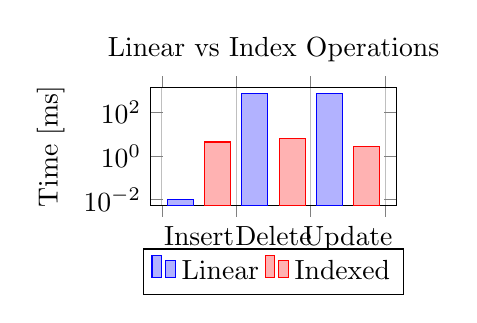
\begin{tikzpicture}
\begin{semilogyaxis}[
	log origin = infty,
	width=4.7cm,height=3.07cm,
    title={Linear vs Index Operations},
        ylabel={Time [ms]},
	symbolic x coords={Insert, Delete, Update, 4},
	x tick label style={
		/pgf/number format/1000 sep=},
	%%ylabel=Time (seconds),
	enlargelimits=0.05,
	legend style={at={(0.5,-0.37)},
	anchor=north,legend columns=-1},
	ybar interval=0.7,
    ]
\addplot
	coordinates {(Insert,.01) (Delete,706.34) (Update,710.77) (4, 1)};
\addplot
	coordinates {(Insert,004.24) (Delete,005.93) (Update,002.68) (4,1)};
    \legend{Linear, Indexed}
\end{semilogyaxis}
\end{tikzpicture}\\
\end{tabular}
\caption{\small Comparison of Linear and Index versions of operators over 100,000 rows of fabricated data. Linear scans do better when more of the data needs to be accessed, but Indexed structures perform far better for small queries.}
\label{figC1}\vspace{.5cm}
    \centering
    \begin{minipage}{.32\textwidth}
        \centering
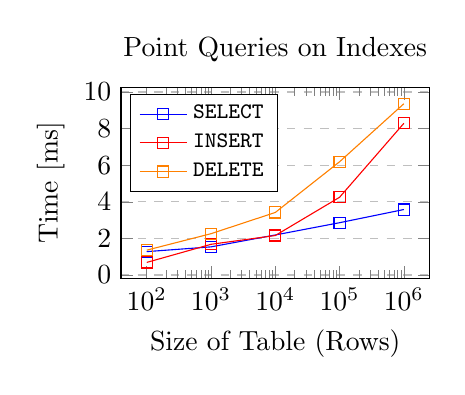
\begin{tikzpicture}
\begin{semilogxaxis}[
    title={Point Queries on Indexes},
        ylabel={Time [ms]},
        	width=5.5cm, height=4cm,
    xlabel={Size of Table (Rows)},
    %xmin=0, xmax=2.5,
    %ymin=0, ymax=.75,
    xtick={100,1000,10000,100000,1000000},
    %ytick={0,.25,.5,.75},
    legend pos=north west,
    ymajorgrids=true,
    grid style=dashed,
    ]
    \addplot[
    color=blue,
    mark=square,
    ]
    coordinates {
    (100,1.28)(1000, 1.54)(10000, 2.19)(100000,2.86)(1000000,3.58)
    };
    \addplot[
    color=red,
    mark=square,
    ]
    coordinates {
    (100,.69)(1000, 1.68)(10000, 2.16)(100000,4.25)(1000000,8.29)
    };
    \addplot[
    color=orange,
    mark=square,
    ]
    coordinates {
    (100,1.36)(1000, 2.26)(10000, 3.42)(100000,6.19)(1000000,9.36)
    };
    \legend{\footnotesize \texttt{SELECT},\footnotesize \texttt{INSERT},\footnotesize \texttt{DELETE}}
\end{semilogxaxis}
\end{tikzpicture}
    \end{minipage}
    \hspace{.2cm}%
    \begin{minipage}{0.64\textwidth}
    \begin{minipage}{.5\textwidth}
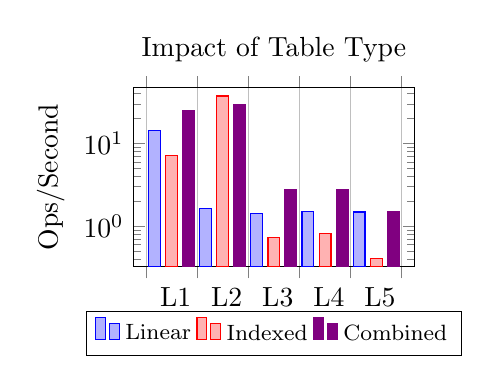
\begin{tikzpicture}
\centering
\begin{semilogyaxis}[
	log origin = infty,
	width=5.15cm, height=3.85cm,
	ybar interval=.7,
	ylabel={Ops/Second},
    title={Impact of Table Type},
	symbolic x coords={\ \ \ L1, \ \ \ L2,  \ \ \ L3,  \ \ \ L4,  \ \ \ L5, 4},
	legend style={at={(0.5,-.25)},
	anchor=north,legend columns=4},
	xtick=data,
	x tick label style={text width=1cm},
	%%ylabel=Time (seconds),
	enlargelimits=0.05,
    ]
\addplot
	coordinates {(\ \ \ L1, 14.401) (\ \ \ L2, 1.622) (\ \ \ L3, 1.424) (\ \ \ L4, 1.499) (\ \ \ L5, 1.486) (4,1)};
\addplot
	coordinates {(\ \ \ L1, 7.081) (\ \ \ L2, 37.539) (\ \ \ L3, .725) (\ \ \ L4, .806) (\ \ \ L5, .408) (4,1)};
\addplot[color=violet, fill=violet]
	coordinates {(\ \ \ L1, 25.240) (\ \ \ L2, 29.682) (\ \ \ L3, 2.765) (\ \ \ L4, 2.768) (\ \ \ L5, 1.485) (4,1)};


\legend{\footnotesize Linear, \footnotesize Indexed, \footnotesize Combined}
\end{semilogyaxis}
\end{tikzpicture}
\end{minipage}
      \begin{minipage}{.5\textwidth}\vspace{.2cm}
\centering
\small
\setlength\tabcolsep{3.5pt}
\begin{tabular}{llllll}
\textbf{Workload}&L1&L2&L3&L4& L5\\\hline
\% Point Reads & 5& 0& 50& 45& 0\\
\% Small Reads & 0& 90& 0& 0& 0\\
\% Large Reads & 5&0&50&45&90\\
\% Insertions& 90& 9& 0& 5& 5\\
\% Deletions & 0& 1& 0& 5& 5\\
\end{tabular}
\end{minipage}
    \end{minipage}
    \begin{minipage}{.32\textwidth}
    		\caption{\small Point queries for Indexed tables of various sizes. Query time grows polylogarithmically in table size.}
		\label{figScaling}
    \end{minipage}\hspace{.2cm}
    \begin{minipage}{.64\textwidth}
    \caption{\small Linear, Indexed, and combined representations of data performing on various workloads over a 100,000 row table. Point reads access 1 record, small reads access 50 records, and large reads access 5\% of the table.}
\label{figworkload}
    \end{minipage}
\end{figure*}
\subsection{Comparison to Sophos}
We compare the performance of \name/'s oblivious index to the searchable symmetric encryption (SSE) scheme Sophos~\cite{Bost16} in Figure~\ref{figSophos}. Sophos does not provide obliviousness guarantees, meaning it leaks access patterns to rows in a table. It does provide a good point of comparison for the performance of our SGX-based oblivious Indexed tables with a non-SGX based, non-oblivious index that still provides some privacy. Sophos only allows search for exact keyword matches via an inverted index, so we compare on simulated data. Specifically, we compare against performance numbers reported in the original Sophos paper for a table of 1.4 million rows and measured using a more powerful machine than ours: an Intel Core i7 4790K 4.00GHz CPU with 8 logical cores, 16GB of RAM, a 250 GB Samsung 850 EVO SSD, running on OS X.10. Despite the difference in hardware and the fact that the Sophos implementation is multithreaded, \name/ outperforms Sophos by 22.6-24.6$\times$ depending on the number of rows returned by a query. We observe that the performance tipping point between Indexed and Linear tables in \name/ arrives between the $10^4$ and $10^5$ rows returned marks in this experiment, and \name/'s performance on larger queries beyond that point would remain constant.

\subsection{Padding Mode Overhead}
\ignore{
\begin{figure}
\small
\centering
\begin{tabular}{llll}
\textbf{Query Type} & \textbf{Obliv} & \textbf{Pad} & \textbf{Overhead} \\\hline
\textbf{Analytic Queries}\\
Aggregate & 0.60s & 2.66s & 4.4$\times$\\%*
Select (Linear) & 1.19s & 2.80s & 2.4$\times$\\%*
Select (Index) & 0.47s & 1.49s & 3.2$\times$\\
Delete (Index) & 0.22s & 0.26s & 1.2$\times$\\
\textbf{Point Queries}\\
Select (Index) & 0.003s & 0.76s & 253$\times$\\
Insert (Index) & 0.011s & 0.013s & 1.2$\times$\\
Delete (Index) & 0.015s & 0.018s & 1.2$\times$\\
\end{tabular}
\caption{\small Overhead of \name/ in padding mode for queries on the CFPB table of 107,000 rows padded to 200,000 rows.}
\label{figPad}
\end{figure}
}

\name/'s padding mode hides not only access patterns to data but also all information regarding the sizes of tables, whether they be at rest in the database, intermediate tables constructed in handling a query, or query results. We evaluated this mode by running queries on the CFPB table of 107,000 rows padded up to 200,000 rows. Our aggregate query over a Linear table had a 4.4$\times$ slowdown and a select had a 2.4$\times$ slowdown. The larger slowdown for aggregates results from the padding algorithm padding to the maximum supported number of groups for aggregates -- in this case, 350,000. We did not evaluate padding mode for Indexed tables because the benefit of Indexed tables results from knowledge of the selectivity of a query, the exact information padding removes by hiding table sizes.

Opaque~\cite{ZDB+17} describes an oblivious padding mode, but does not implement it. To our knowledge, no other comparable system implements an oblivious padding mode, so we are unable to compare to prior work. The results do, however, represent reasonable slowdowns for inflating the size of a table by approximately 2$\times$ with padding.

\subsection{Table Representation Choices}
By providing both Indexed and Linear tables and optimizing queries based on information gained through a first pass over the data, \name/ to makes meaningful performance improvements for diverse queries. To this end, Figure~\ref{figC1} compares the performance of Linear and Indexed tables on \texttt{SELECT} (hash algorithm), \texttt{GROUP BY} (low-cardinality), \texttt{INSERT}, \texttt{DELETE}, and \texttt{UPDATE} queries. Linear scans perform better as the amount of data retrieved from a table increases since the cost of the scan is amortized over more rows, but smaller queries perform significantly better using an index. In general, Indexed \texttt{DELETE} and \texttt{UPDATE} queries significantly outperform Linear tables, but the fast Linear \texttt{INSERT} query -- the one measured in the figure -- outperforms the Indexed \texttt{INSERT}. The performance of linear tables (outside of fast insertions) degrades linearly with the size of the table, but point operations on Indexed tables take time only polylogarithmic in the table size. Figure~\ref{figScaling} shows the running time of insertions, point selections, and point deletions as the size of a table grows by factors of 10. This very gradual increase in running times enables the performance improvements \name/ enjoys over oblivious analytics systems on queries that admit efficacious use of an index.

In some situations, a combined table representation that maintains both an Indexed and Linear table for the same data proves effective. Although \name/ pays insertion and deletion costs for both types of tables to maintain a combined table, it can use the better representation for each query, an important benefit given that many real-world workloads rely heavily on different kinds of reads. Figure~\ref{figworkload} shows \name/ running various workloads with Linear, Indexed, or combined tables. Although there exist cases in which a Linear or Indexed table alone perform best, a combined representation often performs comparably to or much better than either table type alone.
\begin{figure}
\small
\centering
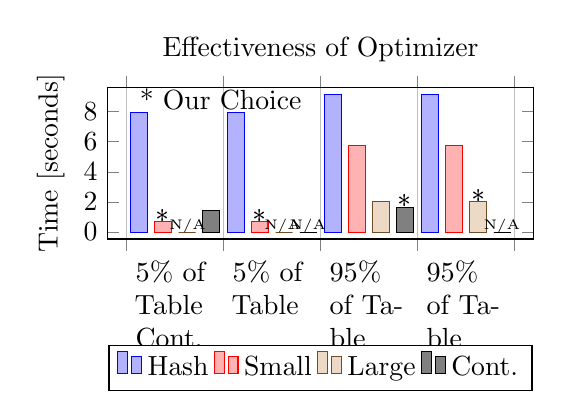
\begin{tikzpicture}
\centering
\begin{axis}[
	width=7cm, height=3.5cm,
	ybar interval=.7,
	ylabel={Time [seconds]},
    title={Effectiveness of Optimizer},
	symbolic x coords={5\% of Table Cont., 5\% of Table, 95\% of Table Cont., 95\% of Table, 4},
	legend style={at={(0.5,-0.7)},
	anchor=north,legend columns=4},
	xtick=data,
	x tick label style={text width=1cm},
	%%ylabel=Time (seconds),
	enlargelimits=0.05,
    ]
\addplot
	coordinates {(5\% of Table Cont., 7.973) (5\% of Table, 7.973) (95\% of Table Cont., 9.123) (95\% of Table, 9.123) (4,1)}; %hash
\addplot
	coordinates {(5\% of Table Cont., .7228) (5\% of Table, .7228) (95\% of Table Cont., 5.732) (95\% of Table, 5.732) (4,1)};	%small
	\addplot
	coordinates {(5\% of Table Cont., 0) (5\% of Table, 0) (95\% of Table Cont., 2.0047) (95\% of Table, 2.0047) (4,1)};	%large
\addplot
	coordinates {(5\% of Table Cont., 1.413) (5\% of Table, 0) (95\% of Table Cont., 1.6313) (95\% of Table, 0) (4,1)};	%cont

\legend{Hash, Small, Large, Cont.}
       \draw (37,108) node {\textasteriskcentered};
       \draw (97,880) node {* Our Choice};
       \draw (137,108) node {\textasteriskcentered};
       \draw (287,204) node {\textasteriskcentered};
       \draw (362.5,238) node {\textasteriskcentered};
       \draw (63,40) node {\tiny{N/A}};
       \draw (161,40) node {\tiny{N/A}};
       \draw (187,40) node {\tiny{N/A}};
       \draw (387,40) node {\tiny{N/A}};

\end{axis}
\end{tikzpicture}
\caption{\small Our optimizer picks the best algorithm for handling \texttt{SELECT} queries based on a preliminary scan that determines whether the data to be returned is small, large, or consists of a continuous set of rows in the table.}
\label{figC3}
\end{figure}

\subsection{Impact of Optimizer}
Figure~\ref{figC3} demonstrates the effectiveness of \name/'s choice of \texttt{SELECT} algorithms, comparing our various algorithms on queries that retrieve 5\% and 95\% percent of a fabricated 100,000 row table. Although the ``Hash'' algorithm performs the best asymptotically, the figure demonstrates that knowledge gleaned only from \name/'s intended leakage about the results of a query (whether it is small/large or a continuous set of rows) suffices to pick an algorithm that will perform much better in practice. Equally impressive gains appear in the choice of \texttt{GROUP BY} algorithm for real queries: the high-cardinality aggregation algorithm used for the query on the USERVISITS table (shown in Figure~\ref{figQueries}) performs 168$\times$ better than the low-cardinality algorithm would on the same query.

\section{Related Work}\label{related}

  \noindent \textbf{Cryptographically-protected database search}.
Fuller et al~\cite{FVY+17} describe prior work on cryptographically-protected databases. The well-known CryptDB~\cite{PRZB12} implements a tradeoff between security and performance, encrypting each field according to its own security needs. More recently, Arx~\cite{PBP16} makes clever use of data structures to allow search over encrypted data. Other solutions, such as Demertzis et al~\cite{DPP+16}, use an inverted index to search encrypted data. These schemes use searchable symmetric encryption (SSE), examples of which include Sophos and Diana~\cite{Bost16, BMO17}. Order-revealing encryption~\cite{BLR+15, LW16} provides encryption for legacy databases.

Several attacks~\cite{IKK12, NKW15, CGPR15, ZKP16} show that inference from context or leakage can compromise schemes in unexpected ways outside their original security models.

  \noindent \textbf{Trusted hardware}.
A number of generic tools provide legacy applications the heightened security available from SGX~\cite{BPH15, STTS17, ATG+16, HZX+16}.
Many works also implement variations of existing systems secured via SGX. M2R~\cite{DSC+15} and VC3~\cite{SCF+15} provide MapReduce and cloud data analytics functionalities, respectively, and Opaque~\cite{ZDB+17} provides secure support for Spark SQL. Like Opaque, Cipherbase~\cite{cipherbase} provides a secure and optionally oblivious variant of Microsoft's SQL Server. SecureKeeper~\cite{BWG+16} uses SGX to build a confidential version of Apache's ZooKeeper (\url{zookeeper.apache.org}). HardIDX~\cite{FBB+17} builds a key-value index in SGX but is not oblivious, and ZeroTrace~\cite{SGF17} provides oblivious memory primitives based on ORAM.

Side channel attacks on SGX make use of page faults~\cite{XCP15, BMD+17}, branch history~\cite{LSG+16}, and thread scheduling~\cite{WKPK16} to learn private information. Recently, Schwarz et al~\cite{SWG+17} run malicious code inside an enclave to attack other enclaves. Other work~\cite{SCNS16, RLT15} closes side channels by making memory traces oblivious or obfuscated. SGX-Shield~\cite{SLK+17} enables address space layout randomization for SGX, and T-SGX~\cite{SLKP17} uses Transactional Synchronization Extensions (TSX) to close side channels.

Intel SGX has also been used to efficiently implement otherwise impractical cryptographic primitives~\cite{FVBG16, NFR+17}. Outside SGX, some other hardware solutions render programs' memory traces oblivious~\cite{CLD16, LHM+15, MLS+13} as well.

  \noindent \textbf{Data Structures over ORAM}. Wang et al.~\cite{WNL+14} develop several general data structures that can be used efficiently on top of ORAM. Roche et al.~\cite{RAC16} design a history-independent ``HIRB tree'' that they build on top of vORAM, an ORAM variant that offers variable-sized blocks.

\section{Conclusion}\label{conclusion}
We have presented \name/, a cryptographically-protected database system using SGX that leaks only table sizes and its query plan (and even hides table sizes in padding mode). We have shown that \name/ handles practical data sets with performance surpassing prior work that had similar or weaker security. We hope practical hardware-based solutions like \name/ can enable rapid progress in private databases and search over encrypted data.

%\section*{Acknowledgements}

{\small \bibliographystyle{acm}
\bibliography{oramsgx}}


%\theendnotes

\end{document}




